\begin{activity} \label{A:11.9.1}  Consider the change of variables
\[x = s + 2 t \ \ \ \ \ \text{ and } \ \ \ \ \ y = 2 s + \sqrt{t}.\]
Let's see what happens to the rectangle $T = [0,1] \times [1,4]$ in the $st$-plane under this change of variable.
	\ba
	\item Draw a labeled picture of $T$ in the $st$-plane.
	
	\item Find the image of the $st$-vertex $(0,1)$ in the $xy$-plane.  Likewise, find the respective images of the other three vertices of the rectangle $T$: $(0,4)$, $(1,1)$, and $(1,4)$.	
	
	\item In the $xy$-plane, draw a labeled picture of the image, $T'$, of the original $st$-rectangle $T$. What appears to be the shape of the image, $T'$?
	
	\item To transform an integral with a change of variable,  we need to determine the area element $dA$ for image of the  transformed rectangle. How would find the area of the $xy$-figure $T'$? (Hint: Remember what the cross product of two vectors tells us.)
	
	\ea

\end{activity}
\begin{smallhint}

\end{smallhint}
\begin{bighint}

\end{bighint}
\begin{activitySolution}
\ba
\item A picture of the rectangle $T$ is shown in the image below.
\item The $st$-vertex $(0,1)$ gets sent to the point $(0+2(1), 2(0)+\sqrt{1}) = (2,1)$ in the $xy$-plane,
\item The point $(0,4)$ in the $st$-plane gets sent to the point $(8,2)$ in the $xy$-plane. The point $(1,1)$ in the $st$-plane gets sent to the point $(3,3)$ in the $xy$-plane.  The point $(1,4)$ in the $st$-plane gets sent to the point $(9,4)$ in the $xy$-plane.
\item The image $T'$ of $T$ is not a rectangle in the $xy$-plane because the change of variable formulas are not linear. The image $T'$ looks like a parallelogram. 
\item The area of $T'$ is the area of a parallelogram, which we can find with a cross product. The sides of the parallelogram can be viewed as the vectors $\vu = \langle 1, 2, 0\rangle$ and $\vv = \langle 6, 1, 0 \rangle$. The area of the parallelogram is then $|\vu \times \vv|$. 
\ea
\begin{center}
\resizebox{!}{1.0in}{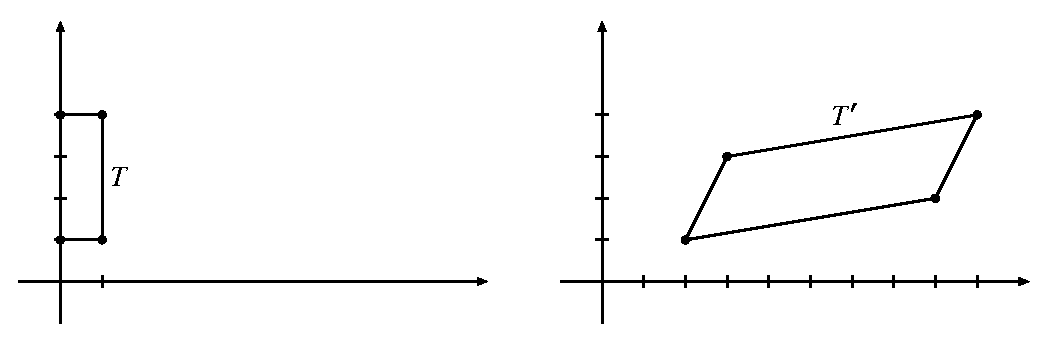
\includegraphics{11_9_Act_1a}}
\end{center}

\end{activitySolution}
\aftera